\documentclass[11pt,a4paper]{scrartcl} % Use scrartcl for support subtitle command

% Hỗ trợ tiếng Việt
\usepackage[utf8]{vietnam}

\usepackage{indentfirst} % Thụt đầu dòng cho tất cả các đoạn văn
\setlength{\parindent}{1cm} % Cài đặt độ thục đầu dòng cho mỗi đoạn, nếu đặt bằng 0pt hoặc 0cm thì coi như không thụt
\setlength{\parskip}{0.5em} % Giãn giữa các đoạn, sẽ scale theo độ rộng của font size

\usepackage{graphicx}

% Tạo các đoạn văn bản minh hoạ
\usepackage{lipsum}


\begin{document}

% Top matter
\title{Homework ?}
\subtitle{Môn học: }
\author{Nguyễn Bùi Nguyên Khoa - MSHV: 2370523}
\date{\today}
\maketitle

% Phần chính, từng câu hỏi
\section{Câu hỏi 1: What ... ?}
\subsection{Đây là phần câu hỏi}
Tại sao Giãn giữa các đoạn, sẽ scale theo độ rộng của font size Cài đặt độ thục đầu dòng cho mỗi đoạn, nếu đặt bằng 0pt hoặc 0cm thì coi như không thụt Thụt đầu dòng cho tất cả các đoạn văn

\subsection{Đây là phần câu trả lời}
Trả lời nhiêu đây là đủ
\lipsum[1-4] % Một vài đoạn văn mẫu
Test location.
\begin{figure}[ht]
    \centering
    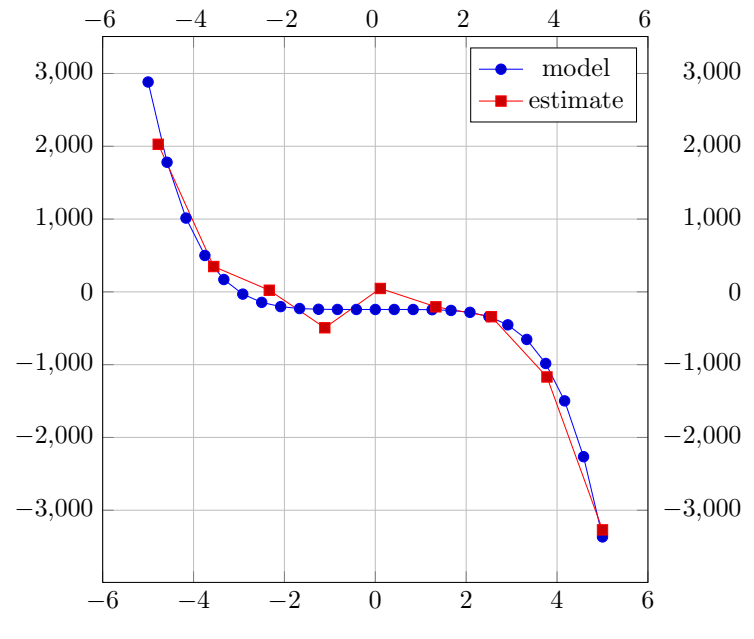
\includegraphics[width=0.75\textwidth]{sample_image.png}
    \caption{An example image}
\end{figure}
\lipsum[6-10] % Thêm một vài đoạn văn mẫu nữa

\section{Câu hỏi 2: Who ... ?}

\section{Câu hỏi 3: Whom ... ?}
\end{document}